% We connect MATLANG with arithmetic circuits as follows.

% We first show that for every MATLANG expression $e$ we can associate a uniform arithmetic circuit family $\{\Phi_n^e\mid n=1,2,\ldots\}$ such that when $I$ is matrix instance of dimension $n$ (or $n\times n$), we can obtain $e(I)$ by evaluating $\Phi_n$ on $I$. \floris{The connection between the dimensions of instances etc and the ``$n$'' in the arithmetic circuits needs to be made precise. E.g., if we have $n^2$ matrices, we need more than $n$ variables...}

We consider circuits over matrices (multiple output gates). We will write 
$\Phi(A_1,\ldots ,A_k)$, where $\Phi$ is an arithmetic circuit with multiple output gates, and each 
$A_i$ is a matrix of dimensions $\alpha_i\times \beta_i$, with $\alpha_i,\beta_i \in \{n,1\}$ to denote 
the input matrices for a circuit $\Phi$. We will also write $\ttype(\Phi)=(\alpha,\beta)$, with 
$\alpha,\beta\in \{n,1\}$, to denote the size of the output matrix for $\Phi$. 
When $\{\Phi_n\mid n=1,2,\ldots\}$ is a uniform family of 
arithmetic circuits over matrices, we will assume that the Turing machine for generating $\Phi_n$ also 
gives us the information about how to access a position of each input matrix, and how to access the 
positions of the output matrix, as is usually done when handling matrices with arithmetic 
circuits \cite{Raz02}. The notion of degree is extended to be the sum of the degrees of all 
the output gates. The former will be denoted as $\Phi_{n}[i,j]$ when $\ttype(\Phi)=(n,n)$, 
$\Phi_{n}[i,1]$ when $\ttype(\Phi)=(n,1)$, $\Phi_{n}[1,j]$ when $\ttype(\Phi)=(1,n)$ and 
$\Phi_{n}$ when $\ttype(\Phi)=(1,1)$. Also, when we write $a \oplus b$ we mean 

\begin{center}
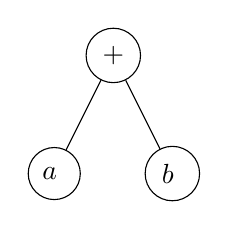
\begin{tikzpicture}[level distance=1.5cm,
  level 1/.style={sibling distance=1.5cm},
  every node/.style = {
  	shape=circle,
    draw,
    align=center,
    top color=white,
    bottom color=white
    }]
  \node {\( + \)}
    child {node { \( a \) }}
    child {node { \( b \) }};
\end{tikzpicture}
\end{center}
When we write $\bigoplus_{l=1}^n a_l$ we mean 

\begin{center}
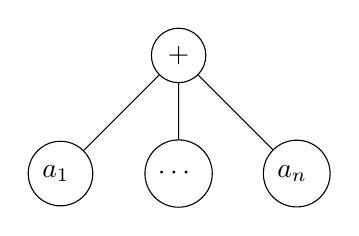
\begin{tikzpicture}[level distance=1.5cm,
  level 1/.style={sibling distance=1.5cm},
  every node/.style = {
  	shape=circle,
    draw,
    align=center,
    top color=white,
    bottom color=white
    }]
  \node {\( + \)}
    child {node { \( a_1 \) }}
    child {node { \( \cdots \) }}
    child {node { \( a_n \) }};
\end{tikzpicture}
\end{center}
Same with $\otimes$. Now we prove the statement.

\newtheorem*{LANGINCIRC}{Theorem~\ref{th-ml-to-circuits}}

\begin{LANGINCIRC}
  Let $e$ be a \langfor expression over a schema $\Sch$, and let $V_1,\ldots ,V_k$ be the variables of $e$ such that $\ttype(V_i)\in \{(\alpha,\alpha), (\alpha,1), (1,\alpha), (1,1)\}$. Then there exists a uniform arithmetic circuit family over matrices $\Phi_n(A_1,\ldots ,A_k)$ such that:
  \begin{itemize}
  \item For any instance $\I = (\dom,\conc)$ such that $\dom(\alpha) = n$ and $\conc(V_i) = A_i$ it holds that:
  \item $\sem{e}{\I} = \Phi_n(A_1,\ldots ,A_k)$.
  \end{itemize}
\end{LANGINCIRC}


\begin{proof}

Let $e$ be a \langfor expression. 

If $e=V$ then $\Phi_n^e:=\Phi(A)$, and we have that
\begin{itemize}
	\item If $\ttype(V)=(1,1)$ then $\ttype(\Phi^e_n)=(1,1)$ and $\Phi^e_n$ has the one input/output gate.
	\item If $\ttype(V)=(1,\alpha)$ then $\ttype(\Phi^e_n)=(1,n)$ and $\Phi^e_n$ has $n$ input/output gates.
  \item If $\ttype(V)=(\alpha,1)$ then $\ttype(\Phi^e_n)=(n,1)$ and $\Phi^e_n$ has $n$ input/output gates.
	\item If $\ttype(V)=(\alpha,\alpha)$ then $\ttype(\Phi^e_n)=(n,n)$ and $\Phi^e_n$ has $n^2$ input/output gates. $\Phi^e_n$ has $n^2$ input/output gates.
\end{itemize}

If $e=e'^T$ then $\Phi^e_n=\Phi^{e'}_n$. 
\begin{itemize}
	\item If $\ttype(\Phi^{e'}_n)=(1, 1)$ then$\Phi^e_n=\Phi^{e'}_n$ and $\type(\Phi^e_n)=(1,1)$.
	\item If $\ttype(\Phi^{e'}_n)=(1, n)$ then $\type(\Phi^e_n)=(n,1)$ and $\Phi^e_n[i,1]:=\Phi^{e'}_n[1,i]$. 
  \item If $\ttype(\Phi^{e'}_n)=(n, 1)$ then $\type(\Phi^e_n)=(1,n)$ and $\Phi^e_n[1,j]:=\Phi^{e'}_n[j,1]$. 
  \item If $\ttype(\Phi^{e'}_n)=(n, n)$ then $\type(\Phi^e_n)=(n,n)$ and $\Phi^e_n[i,j]:=\Phi^{e'}_n[j,i]$. 
\end{itemize}

If $e=e_{\ones}(e')$ where $\ttype(\Phi^{e'}_n)=(\alpha,\beta)$ then $\ttype(\Phi^{e}_n)=(\alpha,1)$ and $\Phi^e_n[i,1]:=1$.

If $e=e_1 + e_2$ we have

\begin{itemize}
	\item When $\ttype(\Phi^{e_1}_n)=\ttype(\Phi^{e_2}_n)=(1, 1)$ is then $\ttype(\Phi^{e}_n)=(1, 1)$ and $\Phi^e_n:=\Phi^{e_1}_n \oplus \Phi^{e_2}_n$.
  \item When $\ttype(\Phi^{e_1}_n)=\ttype(\Phi^{e_2}_n)=(1, n)$ is then $\ttype(\Phi^{e}_n)=(1, n)$ and $\Phi^e_n[1,j]:=\Phi^{e_1}_n[1,j] \oplus \Phi^{e_2}_n[1,j]$.
  \item When $\ttype(\Phi^{e_1}_n)=\ttype(\Phi^{e_2}_n)=(n, 1)$ is then $\ttype(\Phi^{e}_n)=(n, 1)$ and $\Phi^e_n[i,1]:=\Phi^{e_1}_n[i,1] \oplus \Phi^{e_2}_n[i,1]$.
  \item When $\ttype(\Phi^{e_1}_n)=\ttype(\Phi^{e_2}_n)=(n, n)$ is then $\ttype(\Phi^{e}_n)=(n, n)$ and $\Phi^e_n[i,j]:=\Phi^{e_1}_n[i,j] \oplus \Phi^{e_2}_n[i,j]$.
\end{itemize}

If $e=f(e_1, \ldots, e_k)$ we have two cases

\begin{itemize}
  \item When $f$ is retricted to $f_{\odot}$ then
  \begin{itemize}
    \item If $\ttype(\Phi^{e_1}_n)=\ldots =\ttype(\Phi^{e_k}_n)=(1, 1)$ then $\Phi^e_n:=\bigotimes_{l=1}^k \Phi^{e_l}_n$.
    \item If $\ttype(\Phi^{e_1}_n)=\ldots =\ttype(\Phi^{e_k}_n)=(1, n)$ then $\Phi^e_n[1,j]:=\bigotimes_{l=1}^k \Phi^{e_l}_n[1,j]$.
    \item If $\ttype(\Phi^{e_1}_n)=\ldots =\ttype(\Phi^{e_k}_n)=(n, 1)$ then $\Phi^e_n[i,1]:=\bigotimes_{l=1}^k \Phi^{e_l}_n[i,1]$.
    \item If $\ttype(\Phi^{e_1}_n)=\ldots =\ttype(\Phi^{e_k}_n)=(n, n)$ then $\Phi^e_n[i,j]:=\bigotimes_{l=1}^k \Phi^{e_l}_n[i,j]$.
  \end{itemize}
	\item When $f$ is any function, we prove the case when $\ttype(\Phi^{e_1}_n)=\ldots =\ttype(\Phi^{e_k}_n)=(1, 1)$
  (only case necessary). Here $\Phi^e_n$ is 
	
\begin{center}
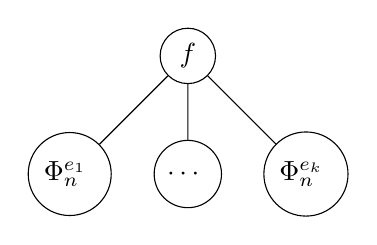
\begin{tikzpicture}[level distance=1.5cm,
  level 1/.style={sibling distance=1.5cm},
  every node/.style = {
  	shape=circle,
    draw,
    align=center,
    top color=white,
    bottom color=white
    }]
  \node {\( f \)}
    child {node { \( \Phi^{e_1}_n \) }}
    child {node { \( \cdots \) }}
    child {node { \( \Phi^{e_k}_n \) }};
\end{tikzpicture}
\end{center}

\end{itemize}

If $e=e_1\cdot e_2$ we have

\begin{itemize}
	\item When $\ttype(\Phi^{e_1}_n)=(1,1)$ and $\ttype(\Phi^{e_2}_n)=(1, 1)$ then $\ttype(\Phi^{e}_n)=(1, 1)$ and $\Phi^{e}_n:=\Phi^{e_1}_n \otimes \Phi^{e_2}_n$.
  \item When $\ttype(\Phi^{e_1}_n)=(1,1)$ and $\ttype(\Phi^{e_2}_n)=(1, n)$ then $\ttype(\Phi^{e}_n)=(1, n)$ and $\Phi^{e}_n[1,j]:=\Phi^{e_1}_n \otimes \Phi^{e_2}_n[1,j]$.
  \item When $\ttype(\Phi^{e_1}_n)=(n,1)$ and $\ttype(\Phi^{e_2}_n)=(1, 1)$ then $\ttype(\Phi^{e}_n)=(n, 1)$ and $\Phi^{e}_n[i,1]:=\Phi^{e_1}_n[i,1] \otimes \Phi^{e_2}_n$.
  \item When $\ttype(\Phi^{e_1}_n)=(n,1)$ and $\ttype(\Phi^{e_2}_n)=(1, n)$ then $\ttype(\Phi^{e}_n)=(n, n)$ and $\Phi^{e}_n[i,j]:=\Phi^{e_1}_n[i,1] \otimes \Phi^{e_2}_n[1,j]$.
  \item When $\ttype(\Phi^{e_1}_n)=(1,n)$ and $\ttype(\Phi^{e_2}_n)=(n, 1)$ then $\ttype(\Phi^{e}_n)=(1, 1)$ and $$\Phi^{e}_n:=\bigoplus_{k=1}^n \left( \Phi^{e_1}_n[1,k] \otimes \Phi^{e_2}_n[k,1] \right).$$
  \item When $\ttype(\Phi^{e_1}_n)=(1,n)$ and $\ttype(\Phi^{e_2}_n)=(n, n)$ then $\ttype(\Phi^{e}_n)=(1, n)$ and $$\Phi^{e}_n[1,j]:=\bigoplus_{k=1}^n \left( \Phi^{e_1}_n[1,k] \otimes \Phi^{e_2}_n[k,j] \right).$$
  \item When $\ttype(\Phi^{e_1}_n)=(n,n)$ and $\ttype(\Phi^{e_2}_n)=(n, 1)$ then $\ttype(\Phi^{e}_n)=(n, 1)$ and $$\Phi^{e}_n[i,1]:=\bigoplus_{k=1}^n \left( \Phi^{e_1}_n[i,k] \otimes \Phi^{e_2}_n[k,1] \right).$$
  \item When $\ttype(\Phi^{e_1}_n)=(n,n)$ and $\ttype(\Phi^{e_2}_n)=(n, n)$ then $\ttype(\Phi^{e}_n)=(n, n)$ and $$\Phi^{e}_n[i,j]:=\bigoplus_{k=1}^n \left( \Phi^{e_1}_n[i,k] \otimes \Phi^{e_2}_n[k,j] \right).$$
\end{itemize}

If $e=\ffor{X}{v}e'(X, v)$, then define $\Phi^{\mathbf{0}}$ 
as the zero matrix circuit $\ttype(\Phi^{\mathbf{0}})=(1,1)$ if $\ttype(\Phi^{e'}_n)=(1,1)$ and 
$\ttype(\Phi^{\mathbf{0}})=(n,n)$ if $\ttype(\Phi^{e'}_n)=(n,n)$. Also, $\Phi^{\mathbf{0}}=0$ and
$\Phi^{\mathbf{0}}[i,j]=0$ $\forall i,j$ for each case respectively. Now for $i=1,\ldots, n$, define
$\Phi^{v_i}$ as the circuit such that $\ttype(\Phi^{v_i})=(n,1)$ and $\Phi^{v_i}[i,1]:=1$ and zero otherwise.
Finally, define

$$\Phi^{e}_n=\Phi^{e'}_n\left( \Phi^{e'}_n \left( \cdots \left( \Phi^{e'}_n\left( \Phi^{\mathbf{0}}, \Phi^{v_1}\right), \Phi^{v_2}\right)\cdots, \Phi^{v_{n-1}} \right), \Phi^{v_n} \right).$$

Note that every circuit adds a constant number of layers except when $e=\ffor{X}{v}e'(X, v)$. 
This means that the depth still is polynomial. When $e=\ffor{X}{v}e'(X, v)$
we have that the depth of the circuit is $n\cdot p(n)$, where the depth of $e'(X, v)$ is $p(n)$, 
so it also remains polynomial.

Here, we do not need to translate scalar multiplication
because it can be simulated using the $\mathsf{ones}$ operator and $f_{\kprod}$ (see section \ref{app:simp}).

\end{proof}

% As a consequence, blah blah....

% In general, uniform arithmetic circuit family $\{\Phi_n^e\mid n=1,2,\ldots\}$ is not necessarily of polynomial degree. Indeed, consider it suffices to consider the MATLANG expression which computes
% $f_n(x)=x^{2^n}$. 
% As uniform arithmetic circuit families of polynomial degree have nice properties, e.g., they can be assumed to be of logarithmic depth, we next want to zoom in such families. In what follows we therefore limit ourselves to MATLANG expressions $e$ such that $\{\Phi_n^e\mid n=1,2,\ldots\}$ is a family of polynomial degree arithmetic circuits.

% \begin{itemize}
% 	\item Checking whether a MATLANG expression $e$ corresponds to a family of of polynomial degree arithmetic circuits is undecidable. 
% \end{itemize}

% Let $e$ be a ``nice'' MATLANG expression, i.e.,  $\{\Phi_n^e\mid n=1,2,\ldots\}$ is a family of polynomial degree arithmetic circuits which can be assumed to be logarithmic depth. 
% \begin{itemize}
% 	\item There exists a MATLANG expression that can
% \end{itemize}

% Let $e$ be a \langfor expression. If $e=V$ we have
% \begin{itemize}
% 	\item When $V$ is $1\times 1$ then $\Phi^e_1$ has the one input/output gate (\textit{not necessary, covered in second item}).
% 	\item When $V$ is $n\times 1$ or $1\times n$ then $\Phi^e_n$ has $n$ input/output gates.
% 	\item When $V$ is $n\times n$ then $\Phi^e_n$ has $n^2$ input/output gates. Here, $V_{ij}=\Phi_n(V)\left[ j+n(i-1)\right]$ and $i,j=1,\ldots, n$ (entries listed row by row).
% \end{itemize}

% If $e=e'^T$ then $\Phi^e_n=\Phi^{e'}_n$. 

% If $e=e_1 + e_2$ we have

% \begin{itemize}
% 	\item When $e$ is $1\times 1$ then $\Phi^e_1$ is $\Phi^{e_1}_1 \oplus \Phi^{e_2}_1$.
% 	\item When $e$ is $n\times 1$ or $1\times n$ then $\Phi^e_n$ has $n$ output gates, where gate $k$ is $\Phi^{e_1}_n[k] \oplus \Phi^{e_2}_n[k]$.
% 	\item When $V$ is $n\times n$ then $\Phi^e_1$ has $n^2$ output gates, where gate $k$ is $\Phi^{e_1}_n[k] \oplus \Phi^{e_2}_n[k]$.
% \end{itemize}

% If $e=f(e_1, \ldots, e_k)$ we have

% \begin{itemize}
% 	\item When $e$ is $1\times 1$ (only case necessary) then $\Phi^e_1$ is 
	
% \begin{center}
% \begin{tikzpicture}[level distance=1.5cm,
%   level 1/.style={sibling distance=1.5cm},
%   every node/.style = {
%   	shape=circle,
%     draw,
%     align=center,
%     top color=white,
%     bottom color=white
%     }]
%   \node {\( f \)}
%     child {node { \( \Phi^{e_1}_1 \) }}
%     child {node { \( \cdots \) }}
%     child {node { \( \Phi^{e_k}_1 \) }};
% \end{tikzpicture}
% \end{center}

% \end{itemize}

% If $e=e_1\cdot e_2$ we have

% \begin{itemize}
% 	\item When $e_1,e_2$ are $1\times 1$ then $\Phi^e_1$ is $\Phi^{e_1}_1 \otimes \Phi^{e_2}_1$.
% 	\item When $e_1$ is $1\times 1$ and $e_2$ is $1\times n$ then $\Phi^e_n$ has $n$ output gates, where output gate $i$ is $\Phi^{e_1}_1 \otimes \Phi^{e_2}_n[i]$.
% 	\item When $e_1$ is $n\times 1$ and $e_2$ is $1\times 1$ then $\Phi^e_n$ has $n$ output gates, where output gate $i$ is $\Phi^{e_1}_n[i] \otimes \Phi^{e_2}_1$.
% 	\item When $e_1$ is $n\times 1$ and $e_2$ is $1\times n$ then $\Phi^e_n$ has $n^2$ output gates, where output gate $k=j + n(i-1)$ is $\Phi^{e_1}_n[i] \otimes \Phi^{e_2}_n[j]$. Note that $k=1,\ldots, n^2$ and $i,j=1,\ldots, n$.
% 	\item When $e_1$ is $1\times n$ and $e_2$ is $n\times 1$ then $\Phi^e_n$ has one output gate $$\bigoplus_{l=1}^n \left( \Phi^{e_1}_n[l] \otimes \Phi^{e_2}_n[l] \right).$$
% 	\item When $e_1$ is $1\times n$ and $e_2$ is $n\times n$ then $\Phi^e_n$ has $n$ output gates, where gate $j$ is $$\bigoplus_{i=1}^n \left( \Phi^{e_1}_n[j] \otimes \Phi^{e_2}_n[j + n(i-1)] \right).$$
% 	\item When $e_1$ is $n\times n$ and $e_2$ is $n\times 1$ then $\Phi^e_n$ has $n$ output gates, where gate $i$ is $$\bigoplus_{j=1}^n \left( \Phi^{e_1}_n[j+n(i-1)] \otimes \Phi^{e_2}_n[j] \right).$$
% 	\item When $e_1$ is $n\times n$ and $e_2$ is $n\times n$ then $\Phi^e_n$ has $n^2$ output gates, where gate $k=j+n(i-1)$ is $$\bigoplus_{l=1}^n \left( \Phi^{e_1}_n[i] \otimes \Phi^{e_2}_n[j+n(l-1)] \right).$$ Note that $k=1,\ldots, n^2$ and $i,j=1,\ldots, n$.
% \end{itemize}

% If $e=\ffor{X}{v}e'(\cI, X, v)$ then $$\Phi^{e}_n=\Phi^{e'}_n\left( \cI, \Phi^{e'}_n \left( \cI, \cdots \Phi^{e'}_n\left( \cI, \Phi^{e'}_n\left( \cI, 0, v_1\right), v_2\right)\cdots, v_{n-1} \right), v_n \right).$$

% Note that every circuit adds a constant number of layers except when $e=\ffor{X}{v}e'(\cI, X, v)$. This means that the depth still is polynomial. When $e=\ffor{X}{v}e'(\cI, X, v)$ we have that the depth of the circuit is $n\cdot p(n)$, where the depth of $e'(\cI, X, v)$ is $p(n)$, so it also remains polynomial.